\documentclass{beamer}\usepackage[]{graphicx}\usepackage[]{color}
% maxwidth is the original width if it is less than linewidth
% otherwise use linewidth (to make sure the graphics do not exceed the margin)
\makeatletter
\def\maxwidth{ %
  \ifdim\Gin@nat@width>\linewidth
    \linewidth
  \else
    \Gin@nat@width
  \fi
}
\makeatother

\definecolor{fgcolor}{rgb}{1, 0.894, 0.769}
\newcommand{\hlnum}[1]{\textcolor[rgb]{0.824,0.412,0.118}{#1}}%
\newcommand{\hlstr}[1]{\textcolor[rgb]{1,0.894,0.71}{#1}}%
\newcommand{\hlcom}[1]{\textcolor[rgb]{0.824,0.706,0.549}{#1}}%
\newcommand{\hlopt}[1]{\textcolor[rgb]{1,0.894,0.769}{#1}}%
\newcommand{\hlstd}[1]{\textcolor[rgb]{1,0.894,0.769}{#1}}%
\newcommand{\hlkwa}[1]{\textcolor[rgb]{0.941,0.902,0.549}{#1}}%
\newcommand{\hlkwb}[1]{\textcolor[rgb]{0.804,0.776,0.451}{#1}}%
\newcommand{\hlkwc}[1]{\textcolor[rgb]{0.78,0.941,0.545}{#1}}%
\newcommand{\hlkwd}[1]{\textcolor[rgb]{1,0.78,0.769}{#1}}%
\let\hlipl\hlkwb

\usepackage{framed}
\makeatletter
\newenvironment{kframe}{%
 \def\at@end@of@kframe{}%
 \ifinner\ifhmode%
  \def\at@end@of@kframe{\end{minipage}}%
  \begin{minipage}{\columnwidth}%
 \fi\fi%
 \def\FrameCommand##1{\hskip\@totalleftmargin \hskip-\fboxsep
 \colorbox{shadecolor}{##1}\hskip-\fboxsep
     % There is no \\@totalrightmargin, so:
     \hskip-\linewidth \hskip-\@totalleftmargin \hskip\columnwidth}%
 \MakeFramed {\advance\hsize-\width
   \@totalleftmargin\z@ \linewidth\hsize
   \@setminipage}}%
 {\par\unskip\endMakeFramed%
 \at@end@of@kframe}
\makeatother

\definecolor{shadecolor}{rgb}{.97, .97, .97}
\definecolor{messagecolor}{rgb}{0, 0, 0}
\definecolor{warningcolor}{rgb}{1, 0, 1}
\definecolor{errorcolor}{rgb}{1, 0, 0}
\newenvironment{knitrout}{}{} % an empty environment to be redefined in TeX

\usepackage{alltt}
\usepackage{../371g-slides}
\title{Correlation \& Simple Regression 1}
\subtitle{Lecture 9}
\author{STA 371G}
\IfFileExists{upquote.sty}{\usepackage{upquote}}{}
\begin{document}
  
  
  

  \frame{\maketitle}

  % Show outline at beginning of each section
  \AtBeginSection[]{
    \begin{frame}<beamer>
      \tableofcontents[currentsection]
    \end{frame}
  }

  %%%%%%% Slides start here %%%%%%%

  \begin{darkframes}
    \begin{frame}{Scatterplots}
      \begin{itemize}
        \item \alert{Scatterplots} are the main graphical tool used to examine the relationship between two variables
        \item The \alert{explanatory} (or \alert{independent}) variable goes on the $X$-axis: it's the variable you want to use to explain observed outcomes
        \item The \alert{response} (or \alert{dependent}) variable goes on the $Y$-axis: it's the variable you want to explain
      \end{itemize}
    \end{frame}

    \begin{frame}{Predicting SAT scores from high school GPA}
      \begin{itemize}
        \item Cases are individual students entering UT in Fall 2000
        \item SAT score is the response variable
        \item High school GPA is the explanatory variable
      \end{itemize}
    \end{frame}

    \begin{frame}[fragile]
\begin{knitrout}
\definecolor{shadecolor}{rgb}{0.137, 0.137, 0.137}\color{fgcolor}\begin{kframe}
\begin{alltt}
\hlkwd{plot}\hlstd{(ut2000}\hlopt{$}\hlstd{GPA, ut2000}\hlopt{$}\hlstd{SAT.C)}
\end{alltt}
\end{kframe}
\includegraphics[width=\maxwidth]{/tmp/figures/unnamed-chunk-3-1} 

\end{knitrout}
    \end{frame}

    \begin{frame}[fragile]
\begin{knitrout}
\definecolor{shadecolor}{rgb}{0.137, 0.137, 0.137}\color{fgcolor}\begin{kframe}
\begin{alltt}
\hlkwd{plot}\hlstd{(ut2000}\hlopt{$}\hlstd{GPA, ut2000}\hlopt{$}\hlstd{SAT.C,} \hlkwc{col}\hlstd{=}\hlstr{"orange"}\hlstd{,} \hlkwc{pch}\hlstd{=}\hlstr{"."}\hlstd{,}
     \hlkwc{xlab}\hlstd{=}\hlstr{"GPA"}\hlstd{,} \hlkwc{ylab}\hlstd{=}\hlstr{"SAT"}\hlstd{)}
\end{alltt}
\end{kframe}
\includegraphics[width=\maxwidth]{/tmp/figures/unnamed-chunk-4-1} 

\end{knitrout}
    \end{frame}

    \begin{frame}{Correlation coefficient}
      \begin{definition}
        The \alert{correlation} $r$ between two variables $X$ and $Y$ measures the strength of the linear relationship between them. Correlation ranges from $-1$ (perfect negative relationship) to $0$ (no relationship) to $1$ (perfect positive relationship).
      \end{definition}
      \pause 
      It is calculated as
      \[ 
        r = \frac{1}{n-1} \sum_{i=1}^n 
        \left( \frac{X_i-\overline{X}}{\text{SD}(X)} \right) 
        \left( \frac{Y_i-\overline{Y}}{\text{SD}(Y)} \right)  
      \]
    \end{frame}

    \begin{frame}[fragile]{How correlation is calculated}
      \[ 
        r = \frac{1}{n-1} \sum_{i=1}^n 
        \underbrace{ \left( \frac{X_i-\overline{X}}{\text{SD}(X)} \right) }_{\text{$z$-score for $i$th GPA}} 
        \cdot
        \underbrace{ \left( \frac{Y_i-\overline{Y}}{\text{SD}(Y)} \right) }_{\text{$z$-score for $i$th SAT}} 
      \]
\begin{knitrout}
\definecolor{shadecolor}{rgb}{0.137, 0.137, 0.137}\color{fgcolor}
\includegraphics[width=\maxwidth]{/tmp/figures/unnamed-chunk-5-1} 

\end{knitrout}
    \end{frame}

    \begin{frame}[fragile]
\begin{knitrout}
\definecolor{shadecolor}{rgb}{0.137, 0.137, 0.137}\color{fgcolor}
\includegraphics[width=\maxwidth]{/tmp/figures/unnamed-chunk-6-1} 

\end{knitrout}
    \end{frame}

    \begin{frame}[fragile]{Calculating correlations in R}
\begin{knitrout}
\definecolor{shadecolor}{rgb}{0.137, 0.137, 0.137}\color{fgcolor}\begin{kframe}
\begin{alltt}
\hlkwd{cor}\hlstd{(ut2000}\hlopt{$}\hlstd{GPA, ut2000}\hlopt{$}\hlstd{SAT.C)}
\end{alltt}
\begin{verbatim}
[1] 0.3904258
\end{verbatim}
\end{kframe}
\end{knitrout}

      \pause

\begin{knitrout}
\definecolor{shadecolor}{rgb}{0.137, 0.137, 0.137}\color{fgcolor}\begin{kframe}
\begin{alltt}
\hlkwd{cor}\hlstd{(ut2000}\hlopt{$}\hlstd{SAT.C, ut2000}\hlopt{$}\hlstd{GPA)}
\end{alltt}
\begin{verbatim}
[1] 0.3904258
\end{verbatim}
\end{kframe}
\end{knitrout}
    \end{frame}

    \begin{frame}{Conditions for correlation}
      In order for correlation coefficients to make sense:
      \begin{itemize}
        \item Both variables must be quantitative
        \item The relationship between $X$ and $Y$ must be linear (i.e., not curved)
        \item There must not be extreme outliers
      \end{itemize}
    \end{frame}

    \begin{frame}{What if the relationship is not linear?}
\begin{knitrout}
\definecolor{shadecolor}{rgb}{0.137, 0.137, 0.137}\color{fgcolor}
\includegraphics[width=\maxwidth]{/tmp/figures/unnamed-chunk-9-1} 

\end{knitrout}
      \pause
      \vspace{-0.5in}
      The correlation is 0 even though there is a strong relationship between $X$ and $Y$!
    \end{frame}

    \begin{frame}{What if there are extreme outliers?}
\begin{knitrout}
\definecolor{shadecolor}{rgb}{0.137, 0.137, 0.137}\color{fgcolor}
\includegraphics[width=\maxwidth]{/tmp/figures/unnamed-chunk-10-1} 

\end{knitrout}

      \pause
      \vspace{0.2in}
      Adding just one outlier makes the correlation jump from 0 to 0.6!
    \end{frame}

    \begin{frame}{Correlation $\neq$ causation}
      \begin{itemize}[<+->]
        \item Just because the correlation between $X$ and $Y$ is large does not mean that $X$ causes $Y$ (or $Y$ causes $X$)
        \item The correlation could be caused by a \alert{lurking variable} that is causing both $X$ and $Y$
        \item Or the correlation could be a coincidence!
      \end{itemize}
    \end{frame}

    \begin{frame}{Lurking variables}
      What could the lurking variable be?
      \begin{itemize}[<+->]
        \item Students with higher GPAs tend to have higher SAT scores
        \item More people tend to drown when ice cream sales are higher
        \item In Europe, more babies tend to be born where there are more storks
      \end{itemize}
    \end{frame}

    \begin{frame}{Seriously, correlation $\neq$ causation, even if $r$ is high}
      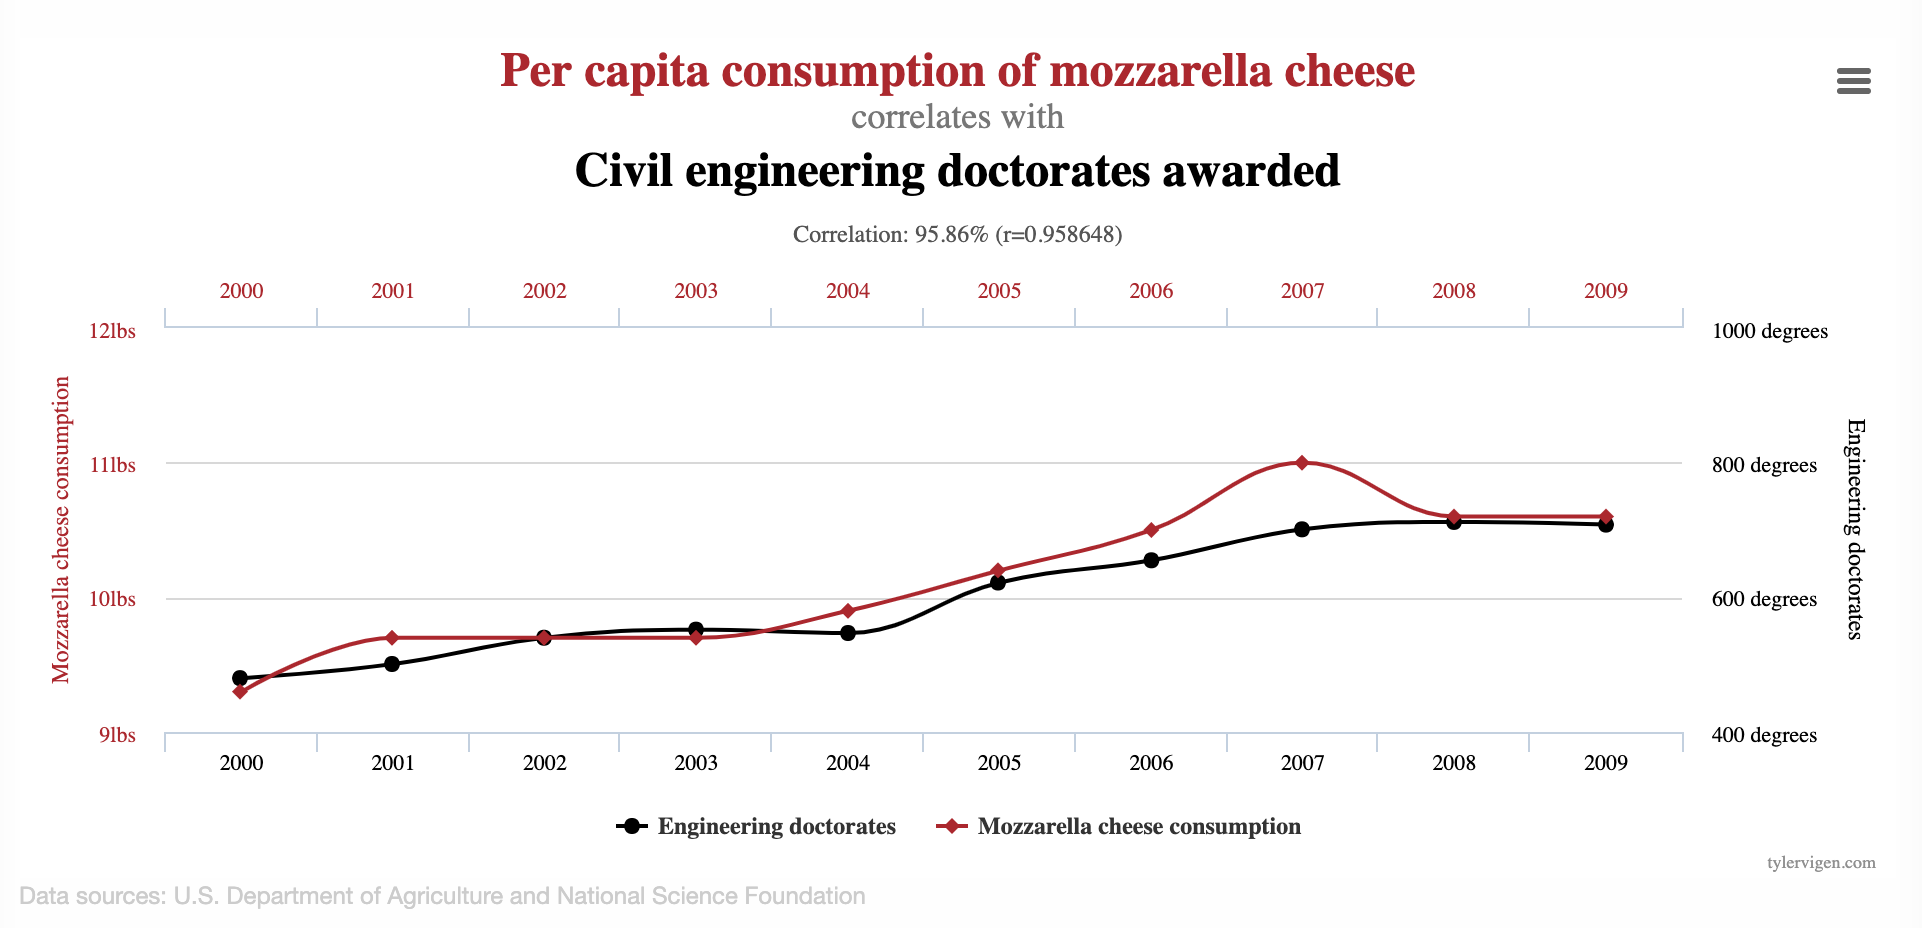
\includegraphics[width=\textwidth]{spurious}
    \end{frame}

    \begin{frame}{Correlation $\neq$ causation}
      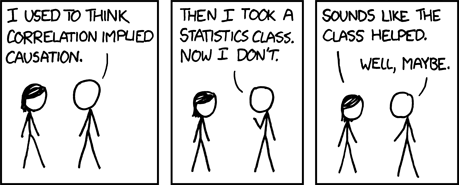
\includegraphics[width=\textwidth]{xkcd}
    \end{frame}
  \end{darkframes}

\end{document}
